\documentclass{article}
\usepackage{graphicx} % Required for inserting images





\documentclass[a4paper,12pt]{article}
\usepackage[utf8]{inputenc}
\usepackage{graphicx}
%  Русский язык
\usepackage{multirow}
\usepackage{wrapfig}
\usepackage[T2A]{fontenc}			% кодировка
\usepackage[utf8]{inputenc}			% кодировка исходного текста
\usepackage[english,russian]{babel}	% локализация и переносы

\usepackage{indentfirst} %Красная строка
\usepackage[a4paper,top=1.3cm,bottom=2cm,left=1.5cm,right=1.5cm,marginparwidth=0.5cm]{geometry}
\usepackage[usenames]{color}
\usepackage{colortbl}
\usepackage{csvsimple}
\usepackage{siunitx}
\usepackage{graphicx}
\graphicspath{ {images/} }
\usepackage{tikz}
\usepackage{pgfplots}

\usepackage{amsmath}
\usepackage{floatflt}
\usepackage[left=20mm, top=20mm, right=20mm, bottom=20mm, footskip=10mm]{geometry}

\usepackage{multicol}
\setlength{\columnsep}{2cm}

\usepackage{multicol}
\setlength{\columnsep}{2cm}
\usepackage{hyperref}


% Заметки
\usepackage{todonotes}

% Математика
\usepackage{amsmath,amsfonts,amssymb,amsthm,mathtools} 
\usepackage{hyperref}

\renewcommand{\AA}{\ensuremath{\mathring{A}}}

\begin{document}
\def\figurename{Рисунок}
\begin{titlepage}
\begin{center}
    {\large МОСКОВСКИЙ ФИЗИКО-ТЕХНИЧЕСКИЙ ИНСТИТУТ (НАЦИОНАЛЬНЫЙ ИССЛЕДОВАТЕЛЬСКИЙ УНИВЕРСИТЕТ)}
\end{center}
\begin{center}
    {\largeФизтех-школа биологической и медицинской физики}
\end{center}

\vspace{1cm}
{\huge
\begin{center}
    {\bf Лабораторная работа по общей физике}\\
    \vspace{0.5cm}
    4.4.1 Амплитудная дифракционная решетка
\end{center}
}

\vspace{4cm}
\begin{flushright}
{\LARGE Выполнила студентка группы Б06-103:\\ Фитэль Алена \\}

\end{flushright}
\vspace{9cm}
\begin{center}
    Долгопрудный, 2023 г.
\end{center}
\end{titlepage}
\newpage
\section{Введение}

\textbf{Цель работы:} знакомство с работой и настройкой гониометра Г5, определение спектральных характеристик амплитудной решетки.

\textbf{В работе используются:} гониометр, дифракционная решетка, ртутная лампа.

\section{Теоретические сведения}

Амплитудную решетку можно представить в виде непрозрачного экрана, в котором прорезано большое число $N$ параллельных щелей - штрихов, расстояние между которыми $d$ (шаг решетки).


Пусть на решетку падает излучение с длиной волны $\lambda$ по нормали к плоскости решетки. Вследствие дифракции лучи, прошедшие через щель в решетке, отклоняются от своего первоначального направления. Рассмотрим лучи, отклонившиеся на угол $\varphi$. Разность хода лучей о эквивалентных точек двух соседних штрихов равна 
\[ \Delta = d \sin \varphi .\]

Если эта величина равна целому числу длин волны:
\begin{equation}
    d \sin \varphi = m \lambda
\end{equation}
то волны взаимно усиливают друг друга.


В соответствии с принципом Гюйгенса–Френеля распределение интенсивности в дифракционной картине определяется суперпозицией волн, приходящих в точку наблюдения от различных щелей решётки. При этом амплитуды всех интерферирующих волн при заданном угле $\varphi$ практически одинаковы, а фазы составляют арифметическую прогрессию.

\[
I = I_0 \dfrac{sin^2[N(kd \sin{\varphi})/2]}{sin^2[(kd \sin{\varphi})/2]},
\]

где $k$~--~волновое число, $I_0$~--~интенсивность волны, идущей от одного штриха. При большом числе щелей свет, прошедший через решётку, распространяется по ряду резко ограниченных направлений. Если на дифракционную решётку падает свет сложного спектрального состава, то после решётки образуется спектр, причём фиолетовые лучи отклоняются решёткой меньше, чем красные (чем больше длина волны, тем сильнее лучи отклоняются решеткой). Входящая в величина $m$ носит название порядка спектра. При $m = 0$ максимумы интенсивности для всех длин волн располагаются при $\varphi = 0$ и накладываются друг на друга. При освещении белым светом нулевой максимум, в отличие от всех прочих, оказывается поэтому неокрашенным. Спектры первого, второго и т.д. порядков располагаются симметрично по обе стороны от нулевого.

\textbf{Угловая дисперсия.} Угловая дисперсия $D$ характеризует угловое расстояние $d \varphi$ между спектральными линиями, отстоящими по длине волны на $d \lambda$:
\begin{equation}
    D=\dfrac{d \varphi}{d \lambda}=\frac{m}{d cos \varphi}=\dfrac{m}{\sqrt{d^{2}-(m \lambda)^{2}}}
\end{equation}

\textbf{Разрешающая способность дифракционной решетки.} Возможность разрешения двух близких спектральных линий зависит от их ширины и от расстояния между ними. Угловое расстояние между двумя близкими спектральными компонентами с длинами волн $\lambda$ и ($\lambda + \Delta \lambda$) равно:
\[
\Delta \varphi =  D d \lambda = \frac{m \Delta \lambda}{d \cos{\varphi}}.
\]
Согласно критерию Рэлея линии становятся неразличимыми, когда расстояние между ними меньше, чем расстояние от максимума одной линии до её первого минимума. Пусть решетка имеет $N$ штрихов. Выберем главный максимум $m$-го порядка для компоненты $\lambda$. Направление на первый дифракционный минимум дается равенством 
\[ d \sin \varphi = \left( m + \dfrac{1}{N} \right) \lambda. \]
По критерию Рэлея это же направление должно соответствовать главному дифракционному максимуму для второй компоненты $\lambda + \Delta \lambda$:
\[ d \sin \varphi = m (\lambda + \Delta \lambda) .\]
Из последних двух равенств находим 
\[\Delta \lambda = \dfrac{\lambda}{mN}.\]
По определению разрешающая способность спектрального прибора $R = \lambda / \Delta \lambda$~--~это отношение длины волны к разности длин волн двух линий, разрешаемых по критерию Рэлея.

Таким образом, приходим к следующему выражению для разрешающей способности дифракционной решетки:
\[R = \lambda / \Delta \lambda = mN .\]
\textbf{Дисперсионная область.} При достаточно широком спектральном интервале падающего света спектры разных порядков могут накладываться друг на друга. Предельная ширина спектрального интервала $ \Delta\lambda$, при которой спектры соседних порядков ($m$ и $m + 1$) перекрываются только своими границами, называется дисперсионной областью $G$. При этом:
\[
d \sin \varphi = m (\lambda + \Delta \lambda) = (m + 1) \lambda
\]
И дисперсионная область:
\[
G = \Delta \lambda = \frac{\lambda}{m}.
\]
\section{Экспериментальная установка}
Принципиальная схема установки для изучения спектров приведена на Рисунке 1. В нашей работе в качестве диспергирующего эелемента используется амплитудная дифракционная решетка, источника света - ртутная лампа со спектром, приведенным на Рисунке 2.  

\begin{figure}[h!]
	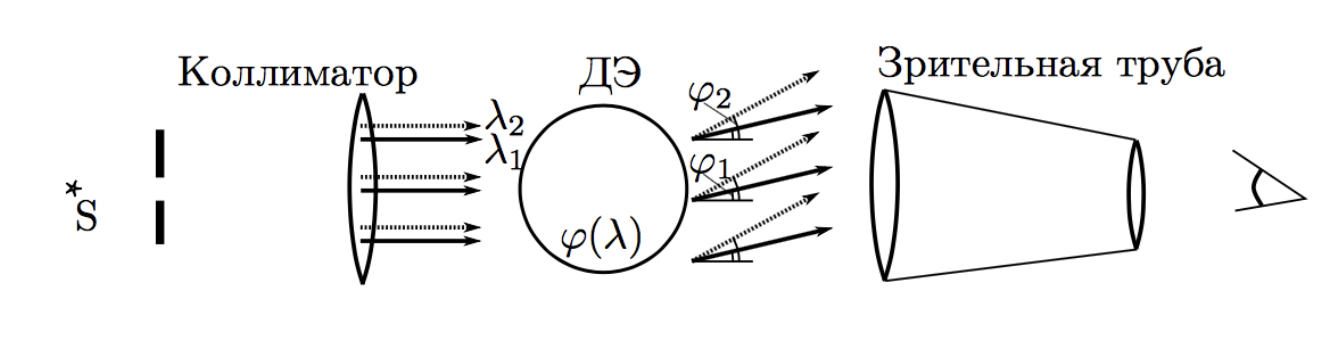
\includegraphics[scale=0.6]{sheme.png}
	\centering
	\caption{Схема прибора: источник-коллиматор–диспергирующий элемент -зрительная труба.}
\end{figure}


\begin{figure}[h!]
	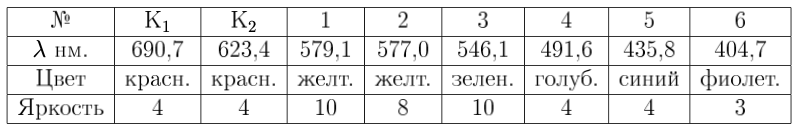
\includegraphics[scale=0.8]{lamp_spectr.png}
	\centering
	\caption{Характеристики спектра ртутной лампы ДРШ.}
\end{figure}

При работе с дифракционной решёткой основной задачей является точное измерение углов, при которых наблюдаются главные максимумы для различных длин волн. В нашей работе для измерения углов используется гониометр Г5, внешний вид которого приведен на Рисунке 3.

\begin{figure}[h!]
	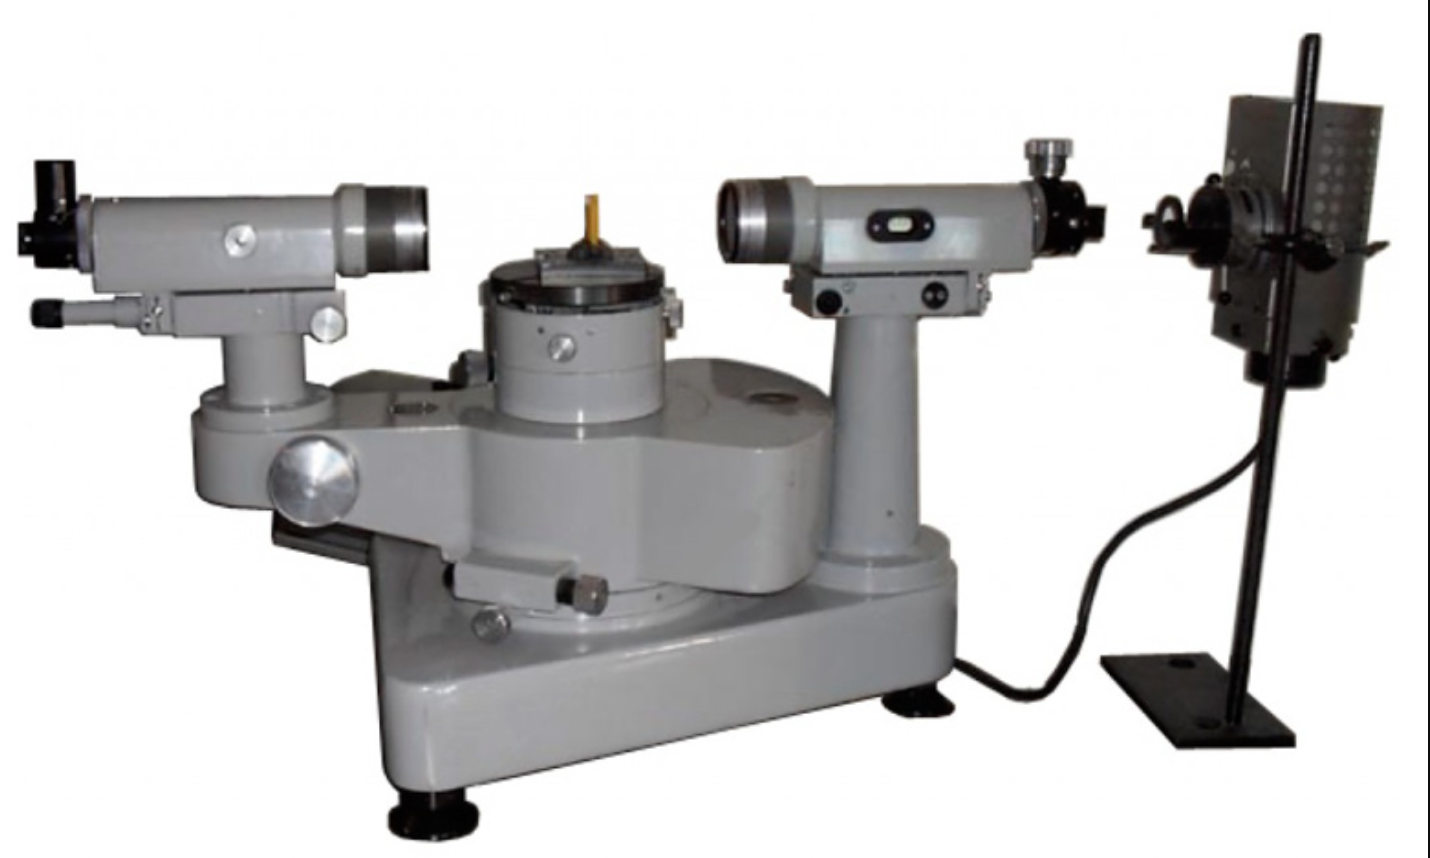
\includegraphics[scale=0.3]{honiometr.png}
	\centering
	\caption{Внешний вид гониометра Г5}
\end{figure}

\newpage

\section{Обработка результатов}
\begin{enumerate}

\item Подберем ширину входной щели коллиматора так, чтобы ширина линий жёлтого
дублета была чуть больше промежутка между линиями двойного штриха окуляра
зрительной трубы. Установим высоту щели, удобную для измерений.Измерим угловые координаты спектральных линий ртути для $\pm 1$ порядка, рассчитаем для них углы дифракции $\varphi_{m}$ и построим график зависимости  $\sin \varphi_{m}$ от длины волны (Рисунок 4). Измеренные и рассчитанные результаты приведены в Таблице 1.


\begin{table}[h!]
\centering{%
\begin{tabular}{|l|cc|cc|cc|cc|}
\hline
 & \multicolumn{2}{c|}{\lambda_{red 1}} & \multicolumn{2}{c|}{\lambda_{red 2}} & \multicolumn{2}{c|}{\lambda_{yellow 1}} & \multicolumn{2}{c|}{\lambda_{yellow 2}} \\ \hline
 & \multicolumn{2}{c|}{690,7\text{ нм}} & \multicolumn{2}{c|}{623,4 \text{ нм}} & \multicolumn{2}{c|}{579,1 \text{ нм}} & \multicolumn{2}{c|}{577 \text{ нм}} \\ \hline
 & \multicolumn{1}{c|}{\varphi} & \sin \varphi & \multicolumn{1}{c|}{\varphi} & \sin \varphi & \multicolumn{1}{c|}{\varphi} & \sin \varphi & \multicolumn{1}{c|}{\varphi} & \sin \varphi \\ \hline
1 & \multicolumn{1}{c|}{18°27'35''} & 0,3167 & \multicolumn{1}{c|}{18°7'4''} & 0,311 & \multicolumn{1}{c|}{17°0'51''} & 0,2926 & \multicolumn{1}{c|}{17°5'21''} & 0,2939 \\ \hline
-1 & \multicolumn{1}{c|}{17°58'14''} & 0,3085 & \multicolumn{1}{c|}{17°38'46''} & 0,3031 & \multicolumn{1}{c|}{16°40'16''} & 0,2869 & \multicolumn{1}{c|}{16°36'13''} & 0,2857 \\ \hline
 & \multicolumn{2}{c|}{\lambda_{green}} & \multicolumn{2}{c|}{\lambda_{blue}} & \multicolumn{2}{c|}{\lambda_{dark blue}} & \multicolumn{2}{c|}{\lambda_{purple}} \\ \hline
 & \multicolumn{2}{c|}{546,1 \text{ нм}} & \multicolumn{2}{c|}{491,6 \text{ нм}} & \multicolumn{2}{c|}{435,8 \text{ нм}} & \multicolumn{2}{c|}{404,7 \text{ нм}} \\ \hline
 & \multicolumn{1}{c|}{\varphi} & \sin \varphi & \multicolumn{1}{c|}{\varphi} & \sin \varphi & \multicolumn{1}{c|}{\varphi} & \sin \varphi & \multicolumn{1}{c|}{\varphi} & \sin \varphi \\ \hline
1 & \multicolumn{1}{c|}{15°55'34''} & 0,2741 & \multicolumn{1}{c|}{14°25'24''} & 0,2491 & \multicolumn{1}{c|}{12°45'38''} & 0,2206 & \multicolumn{1}{c|}{11°48'48''} & 0,2047 \\ \hline
-1 & \multicolumn{1}{c|}{15°42'10''} & 0,2706 & \multicolumn{1}{c|}{14°7'32''} & 0,2441 & \multicolumn{1}{c|}{12°30'28''} & 0,2166 & \multicolumn{1}{c|}{11°35'53''} & 0,201 \\ \hline
\end{tabular}%
}
\caption{Спектр первого  и минус первого порядков}
\label{tab:my-table}
\end{table}

\begin{figure}[h!]
	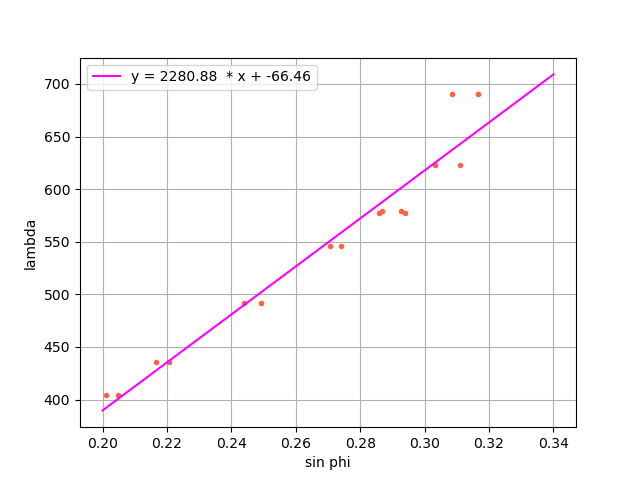
\includegraphics[scale=0.6]{graph 1.png}
	\centering
	\caption{График зависимости $\sin \varphi $ от $\lambda$}
\end{figure}

\item По углу наклона графика прямой из предыдущего пункта с помощью формулы (1)  найдем значение шага решетки:
\[
d = \pm \frac{\lambda}{\sin \varphi} = 2.28 \pm 0.13\text{ мкм}
\]
\item Для оценки угловой дисперсии решетки определим угловые координаты линий желтой пары во всех видимых порядках спектра, положительных и отрицательных. Рассчитаем экспериментальную угловую дисперсию для желтой пары в спектрах разных порядков по формуле:
\[
D = \frac{\Delta \varphi }{\Delta \lambda},
\]
где $\Delta \lambda = 21 \AA$. Измеренные и рассчитанные результаты приведены в Таблице 2. 

\begin{table}[h!]
\centering{%
\begin{tabular}{|l|l|l|l|l|l|l|}
\hline
m & 2 & -2 & 3 & -3 & 1 & -1 \\ \hline
D, \text{ угл. секунды/ангстрем} & 27,9 & 38,3 & 62,8 & 52,5 & 12,9 & 11,6 \\ \hline
\delta \varphi  \text{ угл. секунды} & 585 & 805 & 1319 & 1103 & 270 & 243 \\ \hline
\end{tabular}%
}
\caption{Угловая дисперсия в спектрах разного порядка, определенная по линиям желтого дуплета}
\label{tab:my-table}
\end{table}

\item По данным предыдущего пунка построим график зависимости $D = f(m)$ (Рисунок 5).  По графику определим коэффициент пропорциональности между $D$ и $m$ и сравним его с теоретическим, расчитанным по формуле (2) для длины волны желтой пары:


\[k_\text{эксп} = (13.0 \pm 1.1~\text{угл.сек/ангстрем} = (630 \pm 50) \frac{1}{\text{мм}}\]
\[k_\text{теор} =\frac{1}{\sqrt{d^{2}-\lambda^{2}}} \approx 520 \frac{1}{\text{мм}}\]

\begin{figure}[h!]
	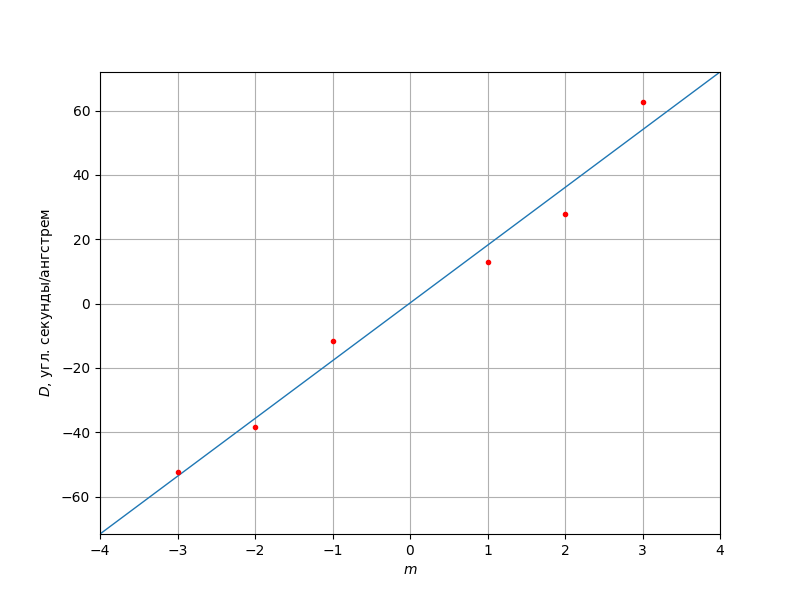
\includegraphics[scale=0.6]{Figure_22.png}
	\centering
	\caption{График зависимости $D = f (m)$}
\end{figure}
\item Определим экспериментальную разрешающую способность по измерениям координаты и угловой ширины желтой линии:
\[
\delta \varphi_{-1} = 28 \text{ угл. секунд} \hspace{1cm}
\delta \varphi_{1} = 35 \text{ угл. секунд}
\]
Усредненная ширина спектра:
\[
\delta \varphi = 32 \pm 4 =  \text{угл. секунд}\]
Тогда расчитаем экспериментальную разрешающую способность:
\[R = \dfrac{\lambda}{\delta \lambda} = \dfrac{D\lambda}{\delta \varphi} \approx 11400\]
Сравнивая полученный результат с теоретическим,расчитанным по формуле $R = mN$, оценим число эффективно работающих штрихов и размер освещенной части решетки:

 \begin{center}
        $N \approx 11400 $ \hspace{1cm} $ d_{work} \approx 2.28\text{ см} $
    \end{center}
\item Рассчитаем порядок спектра, при котором фиолетовая линия наложится на желтую, используя формулу (1):
\[ \dfrac{m_\text{ф}}{m_\text{ж}} = \dfrac{\lambda_\text{ж}}{\lambda_\text{ф}} = 1.43 \approx 10/7\]

\section{Обсуждение результатов и вывод}

В ходе работы были исследованы спектральные характеристики амплитудной решетки с помощью устройства гониометра.
\begin{itemize}
    \item С помощью измерения спектральных линий ртути в $\pm 1$ порядках было расчитано значение шага решетки, которое в пределах погрешности совпадает с указанным на приборе значением ($d_{measured} = 2.28 \pm 13 \text{мкм}, d_{real} = 2 \text{мкм} $). 
    \item  Были проведены измерения угловой дисперсии дифракционной решетки в спектрах разного порядка по линиям жетого дуплета, по которым был определен коэффициент пропорциональности между $D$ и $m$, который несколько превышает теоретическое значение.
    \item Была определена экспериментальная разрешающая способность прибора, оценено число эффективно работающих штрихов и размер освещенной области решетки.
    \item Был рассчитан порядок спектра, при котором произвойдет первое наложение фиолетовой линии на желтую.
\end{itemize}



\end{enumerate}

\end{document}
